\chapter{Method}
\label{sec:method}
As explained in \Cref{sec:introduction} the aim of this work is to find a drone
design that is the result of an optimization problem, which tends to maximize the
MAV's omni-directionality, flight efficiency and controllability. In order to achieve
this goal, it is, first of all, important to state which parameters will be used to
define the design of an MAV. These parameters are defined as:

\begin{itemize}
\item $\beta_{arm}$  (angles formed by the arms with the horizontal plane see \Cref{fig:drone_design})
\item $\theta_{arm}$ (angles formed by the arms in the horizontal plane see \Cref{fig:drone_design})
\item $L$ (arm length)
\item $n$ (number of propellers)
\end{itemize}
\begin{figure}[!h]
  \resizebox{\textwidth}{!}{\begin{subfigure}[b]{0.5\textwidth}
    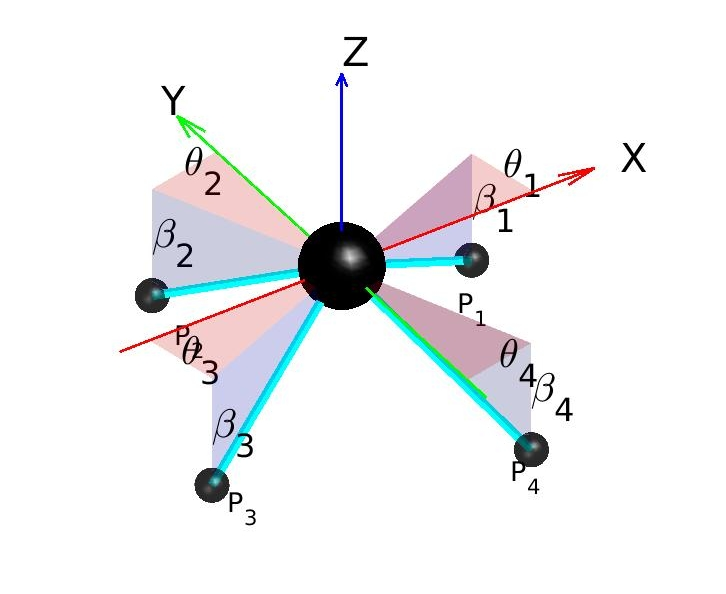
\includegraphics[width=\linewidth]{images/drone_design.jpg}
    \caption{General view.} \label{fig:Quad_3d}
  \end{subfigure}
  \hspace*{\fill} % separation between the subfigures
  \begin{subfigure}[b]{0.45\textwidth}
    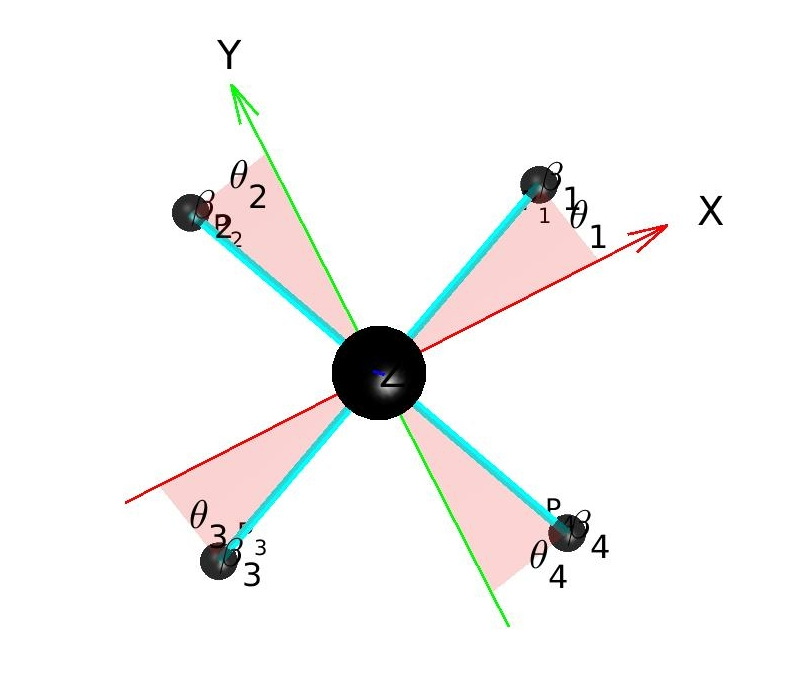
\includegraphics[width=\linewidth]{images/drone_design1.jpg}
    \caption{Top view.} \label{fig:Quad_up}
  \end{subfigure}
  \hspace*{\fill} % separation between the subfigures
  \begin{subfigure}[b]{0.55\textwidth}
    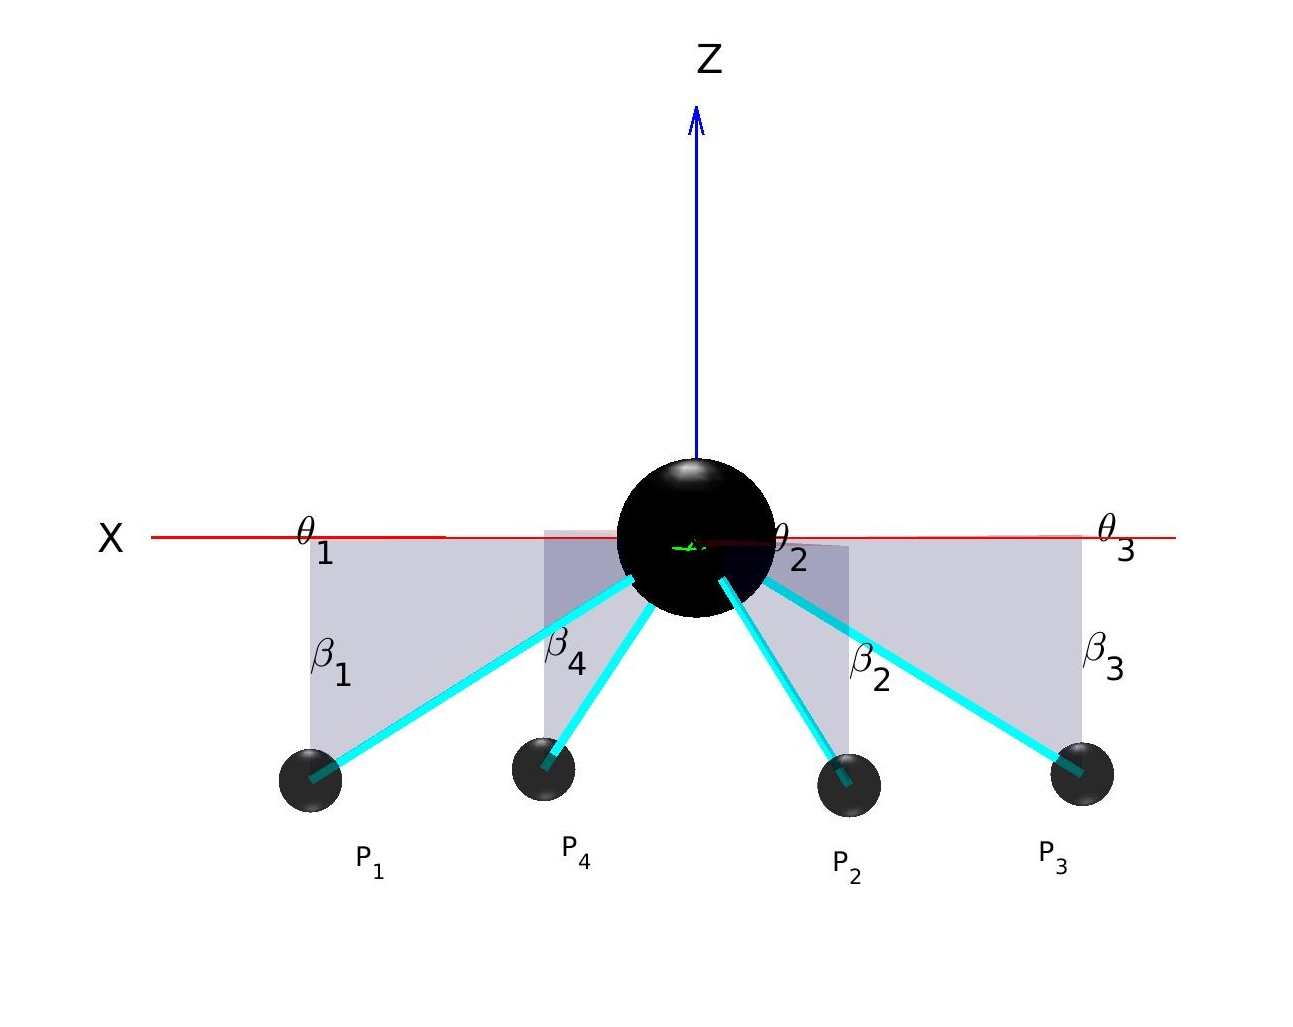
\includegraphics[width=\linewidth]{images/drone_design2.jpg}
    \caption{Side view.} \label{fig:Quad_side}
  \end{subfigure}}
  \caption{Arbitrairy quad-copter design to illustrate the parameters that define the morphology of an
  MAV (with $n = 4$, $\beta_{arm}\ =\ [30^{\circ}, 30^{\circ}, 30^{\circ}, 30^{\circ}]$,
  $\theta_{arm}\ =\ [22^{\circ}, 22^{\circ}, 22^{\circ}, 22^{\circ}]$, and $L\ =\ 0.4\ [m]$).}
  \label{fig:drone_design}
\end{figure}

To solve the problem, an optimization software or tool is developed with
MATLAB$^\textrm{\textregistered}$\footnote{\resizebox{\textwidth}{!}{A numerical computing environment and
programming language developed by MathWorks$^\textrm{\textregistered}$ \citep{noauthor_matlab_2018}.}}.
This tool returns the aforementioned parameters along with other information on
the corresponding MAV design. The interesting drone designs which result from the tool are then simulated on
Gazebo$^\textrm{\textregistered}$\footnote{An open source robot simulation software \citep{noauthor_gazebo_nodate}.}
and the control of the different models is achieved using a Robotic Operating
System\footnote{An open source collection of software that help developers to
create robot applications \citep{rostutorials}.} (ROS) node.\\
This chapter first covers the theory needed to obtain a generalized mathematical
model for a n-rotor MAV with an arbitrary morphology. Then, the optimization
problem is defined. Afterwards, the optimization tool is described. In the end,
the theoretical background needed to perform the simulations is covered.

\section{Modelisation of MAVs}
\label{sec:modeling_mav}
In the following part, a dynamical model for a general design of an MAV is presented.
Such a modelisation is needed to mathematiacally optimize the morphology of
an MAV. This model is inspired by the models presented in
\citep{kamel_voliro:_2018} and \citep{ryll_modeling_2012}.

\subsubsection{Assumptions}
\label{sec:assumptions}
In this model, the first assumption is that the MAV is composed of n+1 rigid bodies:
one for each propeller unit $P_i$ and one for the body B. Then, it is considered that
the thrust is produced by irreversible fixed-pitch motor-propeller actuators. Finally,
only the aerodynamic forces and torques that are responsible for the MAV actuation
are considered, all the second order effects and disturbances are neglected as well as
the airflow interactions between the rotors are neglected.

\subsubsection{Initial Definitions}
\label{sec:definitions}
In order to understand correctly the dynamical model, a few definitions are
needed. First, let us define $\mathcal{F}_{W} : \{O_{W}; X_{W},  Y_{W},  Z_{W}\}$
as the world fixed inertial frame and $\mathcal{F}_{B}: \{O_{B}, X_{B},  Y_{B},
Z_{B}\}$
as a moving frame attached to the MAV. Also, $\mathcal{F}_{P_{i}} : \{O_{P_{i}};
X_{P_{i}}, Y_{P_{i}},  Z_{P_{i}}\}, i = 1...n$ is the frame of the i-th propeller.
The propeller rotates around the axis $Z_{P_{i}}$, and thus the thrust $T_{i}$ is
produced along this axis. The tilt movement of the rotors is a simple rotation
around $X_{P_{i}}$. Now let $^{W}R_{B}$ be the orientation of the body frame
with respect to the world frame and $^{B}R_{P_{i}}$ be the orientation of the
i-th propeller with respect to the body frame. It is
straightforward with the help of \Cref{fig:tilt_model} that

\begin{equation}
  \label{rot_b_pi}
  ^{B}R_{P_{i}} \ = \ R_{Z}\bigg((i-1)\frac{2\pi}{n}\bigg) R_Z(\theta_{arm,i})
  R_Y(\beta_{arm,i}) R_{X}(\alpha_{i}),\  i = 1...n\, .
\end{equation}

Equivalently, let

\begin{equation}
  \label{O_pi}
  ^{B}O_{P_{i}} \ = \ R_{Z}\bigg((i-1)\frac{2\pi}{n}\bigg) R_Z(\theta_{arm,i}) R_Y(\beta_{arm,i})
  \begin{bmatrix}
    L \\
    0 \\
    0
  \end{bmatrix}
  ,\   i = 1...n \,
\end{equation}

be the origin of the i-th propeller frame  $\mathcal{F}_{P_{i}}$.
In \Cref{rot_b_pi} and (\ref{O_pi}), $(i-1)\frac{2\pi}{n}$ is the angle that
the i-th arm would form with axis $X_B$ if the arms of the drone are evenly
distributed in the horizontal plane, $\theta_{arm,i}$ is the angle that i-th arm forms
in the horizontal plane with respect to its evenly distributed position
(see \Cref{fig:drone_design}), $\beta_{arm,i}$ is the angle that the i-th arm forms with
the horizontal plane (see \Cref{fig:drone_design}), $\alpha_{i}$ is the tilting
angle of the i-th propeller about the $X_{P_{i}}$ axis, L is the arm length and
n is the number of propellers.

\begin{figure}[!h]
  \centering
  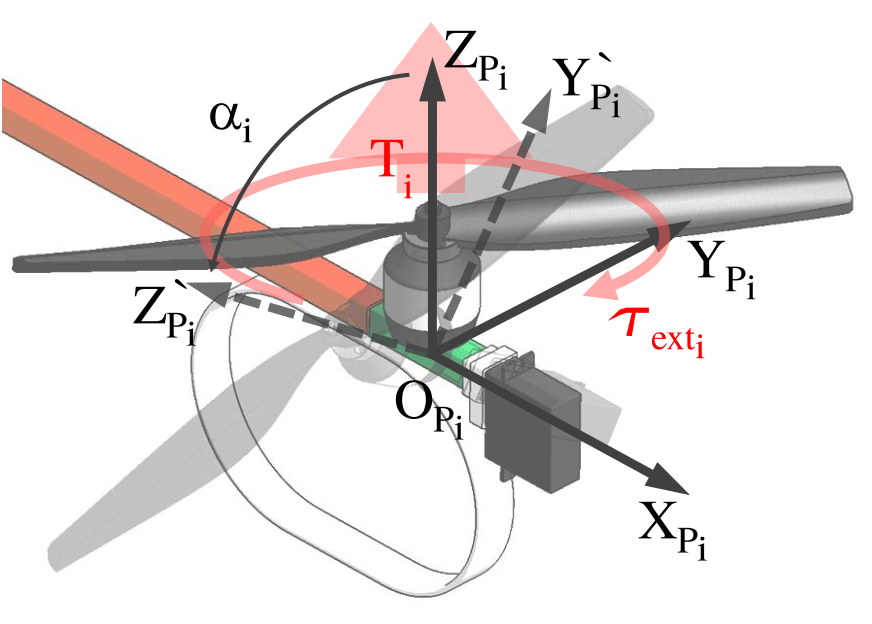
\includegraphics[width=0.45\textwidth]{images/tilt_model.png}
  \caption{Representation of the i-th tilting arm \citep{ryll_modeling_2012}.}
  \label{fig:tilt_model}
\end{figure}

\subsubsection{Equations of motion}
\label{sec:equations}
Using Newton-Euler formalism, the general equations of motion of the MAV are
\begin{equation}
  \label{acc_eq}
  \begin{cases}
    \dot{\omega}_B  \ = \ I_B^{-1} \sum_{i=1}^{n}  \big(\ ^{B}R_{P_{i}} \tau_{ext,i} + \tau_{Bi} \ \big) \, ,\\
    \ddot{p}  \ = \
    \begin{bmatrix}
      0 \\
      0 \\
      -g
    \end{bmatrix}
    \frac{1}{m} \ ^{W}R_B \sum_{i=1}^{n} T_i \, .
  \end{cases}
\end{equation}

Where

\begin{equation}
  \label{tau_b_i}
  \tau_{Bi}  \ = \ ^{B}O_{P_{i}} \times\   ^{B}R_{P_{i}} T_{P,i}\, ,
\end{equation}

\begin{equation}
  \label{tau_ext_i}
  \tau_{ext,i}  \ = \  \big[0, \ \  0, \ \  - c_i \kappa_m w_i^2 \big]^T \, ,
\end{equation}

\centerline{ $\begin{cases} c_i = 1, & \mbox{if } i \mbox{ is odd } (cw\ rotation\ to
\ produce + thrust)\\ c_i = -1 & \mbox{if } i\mbox{ is even } (ccw\ rotation\ to
\ produce + thrust) \end{cases}$ }

and

\begin{equation}
  \label{T_i}
  T_i  \ = \ ^{B}R_{P_{i}} T_{Pi} \, ,\ \ T_{Pi}  \ = \ \big[0, \ \ 0, \ \
  \kappa_f w_i^2 \big]^T\, .
\end{equation}

In \Cref{acc_eq} $g$ is the gravity constant, in \Cref{tau_ext_i} $\kappa_{m}$
is the propeller drag coefficient, in \Cref{T_i} $\kappa_{f}$ is the propeller
thrust coefficient and in \Cref{tau_ext_i} and (\ref{T_i}) $w_{i}$ is the i-th
propeller rotation speed.
The force and torque that the drone produces in body frame $\mathcal{F}_B$ are

\begin{equation}
  \label{force_eq}
    \begin{bmatrix}
      M_B \\
      F_B
    \end{bmatrix} \ = \
    \begin{bmatrix}
      \sum_{i=1}^{n}  \big(\ ^{B}R_{P_{i}} \tau_{ext,i} + \tau_{Bi} \ \big) \\
      \sum_{i=1}^{n} T_i
    \end{bmatrix}
    \, ,
\end{equation}

that can be rewritten

\begin{equation}
  \label{force_eq_alloc}
    \begin{bmatrix}
      M_B \\
      F_B
    \end{bmatrix} \ = \
    A(\alpha)W
    \, .
\end{equation}

Where $W = [w_1^2,\ w_2^2,\ ...,\ w_n^2]$ and\\\\
\resizebox{\textwidth}{!}{
$A(\alpha) \ = \
\begin{bmatrix}
  (-\kappa_f L s(\beta_{arm,1}) c(\theta_{arm,1}) +c_1\kappa_m s(\theta_{arm,1})) s(\alpha_1)
  + (\kappa_f L s(\theta_{arm,1}) +c_1 \kappa_m c(\theta_{arm,1}) s(\beta_{arm,1})) c(\alpha_1) & ...\\
  (-\kappa_f L s(\beta_{arm,1}) s(\theta_{arm,1}) - c_1 \kappa_m c(\theta_{arm,1})) s(\alpha_1)
  + (-\kappa_f L c(\theta_{arm,1}) +c_1 \kappa_m s(\beta_{arm,1}) s(\theta_{arm,1})) c(\alpha_1) & ...\\
  (-L \kappa_f c(\beta_{arm,1})) s(\alpha_1) +(c_1 \kappa_m c(\beta_{arm,1})) c(\alpha_1) & ...\\
  s(\theta_{arm,1}) \kappa_f s(\alpha_1) + s(\beta_{arm,1}) c(\theta_{arm,1}) \kappa_f c(\alpha_1) & ...\\
  -c(\theta_{arm,1}) \kappa_f s(\alpha_1) +s(\beta_{arm,1}) s(\theta_{arm,1}) \kappa_f c(\alpha_1) & ...\\
  c(\beta_{arm,1}) \kappa_f c(\alpha_1) & ...
\end{bmatrix}$
}\\\\
is the $6 \times n$ allocation matrix and $c(\cdot)$ and $s(\cdot)$ represent the
cosine and sine operator respectively.

\subsubsection{Static allocation}
\label{sec:allocation}
The optimization tool has to compute the maximal reachable force and torque in
a large number of directions. So to compute that in a reasonable time in
\citep{kamel_voliro:_2018} an approach to transform the non-linear allocation matrix
into a static allocation matrix, which renders the problem of inverse kinematic
linear, is presented. To do so, the system in \Cref{force_eq_alloc} is rewritten as

\begin{equation}
  \label{static_force_eq}
    \begin{bmatrix}
      M_B \\
      F_B
    \end{bmatrix} \ = \
    A_{static}F_{dec}
    \, .
\end{equation}
Where $F_{dec}$ is the decomposed force vector defined as follow
\begin{equation}
  \label{f_dec}
    F_{dec} \ = \
    \begin{pmatrix}
      F_{h,1} \\
      F_{v,1} \\
      ... \\
      F_{h,n} \\
      F_{v,n}
    \end{pmatrix} \, ,
\end{equation}

with $F_{v,1}\ = \ \kappa_f cos(\alpha_i)$ the vertical force produced by the i-th
propeller and $F_{h,1}\ = \ \kappa_f sin(\alpha_i)$ the horizontal force produced
by the i-th propeller. And the static matrix defined as\\\\
\resizebox{\textwidth}{!}{
$A_{static} \ = \
\begin{bmatrix}
      -\kappa_f L s(\beta_{arm,1}) c(\theta_{arm,1}) +c_1\kappa_m s(\theta_{arm,1})  &
      + \kappa_f L s(\theta_{arm,1}) +c_1 \kappa_m c(\theta_{arm,1}) s(\beta_{arm,1})  & ... & ...\\
      -\kappa_f L s(\beta_{arm,1}) s(\theta_{arm,1}) - c_1 \kappa_m c(\theta_{arm,1}) &
      -\kappa_f L c(\theta_{arm,1}) +c_1 \kappa_m s(\beta_{arm,1}) s(\theta_{arm,1})  & ... & ...\\
      -L \kappa_f c(\beta_{arm,1}) & c_1 \kappa_m c(\beta_{arm,1})  & ... & ...\\
      s(\theta_{arm,1}) \kappa_f & s(\beta_{arm,1}) c(\theta_{arm,1}) \kappa_f & ... & ...\\
      -c(\theta_{arm,1}) \kappa_f  & s(\beta_{arm,1}) s(\theta_{arm,1}) \kappa_f & ... & ...\\
      0 & c(\beta_{arm,1}) \kappa_f  & ... & ...
\end{bmatrix}$
}\\\\
a $6 \times 2n$ matrix that is invariant for a drone design. Using the Moore-Penrose
pseudo inverse we can easily get the inverse kinematic as

\begin{equation}
  \label{inverse_kin}
  F_{dec}  \ = \ A_{static}^{\dagger}
    \begin{bmatrix}
      M_{des} \\
      F_{des}
    \end{bmatrix}
    \, .
\end{equation}

Which returns the decomposed force vector for a desired force and torque. Finding
the tilting angles and propellers rotation speed required to attain this desired
force and torque is then

\begin{equation}
  \label{decomposition}
  \begin{cases}
    w_i^2 = \frac{1}{\kappa_f} \sqrt{F_{v,i}^2 + F_{h,i}^2} \\
    \alpha_i = atan2(F_{h,i},F_{v,i})
  \end{cases}\, .
\end{equation}

\section{Optimization problem}
\label{sec:optimization_problem}
The following section focuses on the optimization problem that the tool has to
solve in order to obtain a MAV design that is optimal. The criteria that make
this design optimal are also discussed.

\subsubsection{Problem statement}
\label{sec:problem}
 The optimization problem is stated as follow

\begin{equation}
  \label{opt_pb}
  \begin{aligned}
    & \underset{x}{\text{arg max}}
    & & f(x) &\text{subject to} &
    \begin{cases}
      c(x) \leq 0 \\
      ceq(x) = 0 \\
      A\cdot x \leq 0 \\
      Aeq \cdot x = 0 \\
      lb \leq x \leq ub\, ,
    \end{cases}
  \end{aligned}
\end{equation}

where $f(x)$ is the cost function, $x$ the argument vector, $c(x)$
the non-linear inequality constraint vector, $ceq(x)$ the non-linear equality
constraint vector, $A$ the linear inequality constraint matrix, $Aeq$ the linear
equality constraint matrix, $lb$ the lower bound vector of the arguments ($x$)
and $ub$ the upper bound vector.\\
Once the optimization problem solved, the output is the optimal argument vector
$x^*$ that maximizes the cost function $f(x)$. In our case the argument vector
$x$ is composed of the MAV's morphology parameters ($\beta_{arm}$, $\theta_{arm}$, $L$, $n$)
and the cost functions are the subject of the next section.

\subsubsection{Cost Functions}
\label{sec:cost_functions}
As stated in \Cref{sec:introduction}, the aim of the project is to obtain a multi-rotor
design that is omni-directional. Therefore, it is the heart of the problem to
define meaningful cost functions for the optimization problem, which when
solved will return parameters for an omni-directional drone. In this section,
the few cost functions that capture the omni-directionality are described.\\
The first cost function consists in maximizing the minimal attainable force and
the minimal attainable torque that the MAV can produce in any direction. The
omni-directionality is defined as the drone capacity to accelerate instantaneously
in every direction. In order to do that the MAV has to have high minimal attainable
force and torque, hence this cost function. It turns out that this cost function is also
computationally less demanding for the solver than the others. Indeed, when the multi-rotors applies a
force or torque in the direction parallel to one of its arms, the propeller on this arm
is perfectly unable to produce any force or torque in this direction. This is due to
the fact that no matter what the tilting angle for this propeller is, the thrust it
produces is parallel to the arm direction (see \Cref{fig:tilt_model}). Therefore,
the minimal attainable forces and torques for the drone are in the direction towards which
one of the propeller can't apply any thrust, i.e. the arm directions. So instead of optimizing the force
and torque in a large number of direction, it is enough for this cost function to
optimize the force and torque in $n$ directions.\\
The second cost function consist of maximizing the minimal attainable force
and the minimal attainable torque that the MAV can produce in any direction
and minimizing the MAV’s inertia. It is the same as the first cost function, but
the last term is added in order to have an easier drone to control and thus add
a criterion on the controllability.\\
The next cost function is designed to maximize the volume of the reachable
force and torque space. The force and torque spaces are two polyhedrons formed
by the drone’s attainable forces and torques in every direction (see \Cref{fig:tool_outputa}
and \Cref{fig:tool_outputb}). The idea behind this cost function is to have the
biggest task space for the drone and hence increase the MAV’s ability to navigate
in any orientation and to any position. This cost function is computationally heavy for the solver,
because in order to have precise polyhedrons for the different spaces, the forces and
torques have to be computed in at least 578 directions.\\
Another cost function that maximizes the force, the torque and the hover
efficiency in all directions is developed. The aim of this cost function
is to maximize the agility of the MAV for good disturbance rejection. Moreover,
the term that maximizes the hover efficiency is designed to give the drone
the ability to perform manipulation efficiently in any orientation. Solving the
optimization problem for this cost function can also be computationally heavy
depending on how many effective directions you choose to represent “all directions”.\\
The last cost function maximizes the force and the torque in one defined
direction d. It is mostly designed to test the optimization tool as it is
computationally light and, given specific directions, the optimal design is
pretty straightforward. For instance, if you maximize the force in the $Z$
direction for a 4-rotors MAV, the expected optimal solution would be a traditional
quad-copter.
The presented cost functions use the multi-rotor model described in
\Cref{sec:modeling_mav} to compute the different forces and torques in the
different directions.

\subsubsection{Solver}
\label{sec:solver}
To solve the problem in \Cref{opt_pb}, the tool uses the
MATLAB$^\textrm{\textregistered}$ function fmincon, with different algorithms.
The one showing the quickest convergence and the best results being the sequential
quadratic programming (sqp) algorithm.

\section{Optimization tool}
\label{sec:optimization_tool}
As explained above, an optimization tool has been developed to perform
the design optimization of the drone and return information on the resulting design.
In this section the tool is exposed and its working principle is explained.
\subsubsection{User Guide}
\label{sec:user_guide}
To use the tool, the graphical user interface (GUI) represented in \Cref{fig:gui}
first has to be opened. Then, the parameters to optimize have to be selected. The
choice is between optimizing just $\beta_{arm}$ angles, or $\beta_{arm}$ angles with other
selected parameters (see \Cref{fig:gui}). Afterwards, the design parameters that
are not selected for the optimization have to be specified. For instance, if the arm
length is not to be optimized, the user has to specify an arm length. To solve the
optimization the sqp algorithm needs an initial solution. Hence, an initial solution
is expected from the user. Then the cost function has to be chosen from the list
(see \Cref{fig:gui}). Finally, in order to obtain a result the user only needs to
push the “start optimization” button.

\begin{figure}[!h]
  \centering
  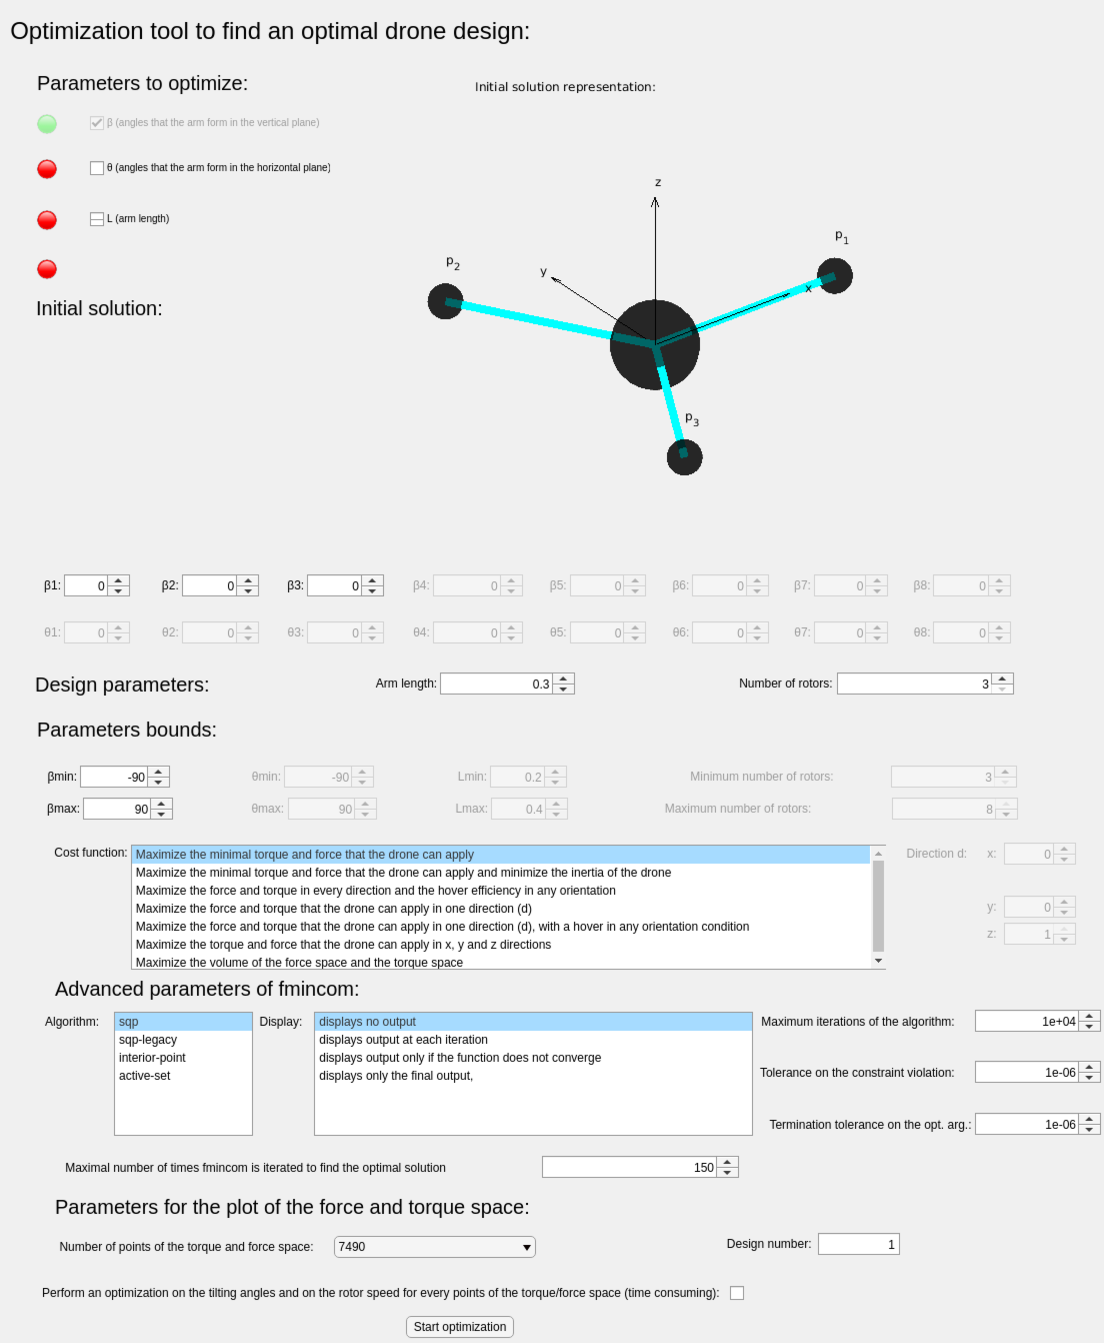
\includegraphics[width=0.8\textwidth]{images/gui.png}
  \caption{MAV morphology optimization tool GUI.}
  \label{fig:gui}
\end{figure}

\subsubsection{Outcome}
\label{sec:outcome}
Apart from the optimal design parameters ($\beta_{arm}$, $\theta_{arm}$, $L$ and $n$), the
optimization tool returns a MATLAB$^\textrm{\textregistered}$ plot containing
the attainable force space, the attainable torque space, the hover efficiency in
every orientation and a schematic of the MAV’s design (see \Cref{fig:tool_output}).
It is important to note that the force and torque space and the hover efficiency
diagram are all represented in the drone’s body frame. And thus, in the force and toque
space diagrams, the dots that can be observed in \Cref{fig:tool_outputa} reprent directions
equally distributed arround the MAV's body center. The distance at which a
point is with respect to the center of the body represents the magnitude of the maximal
force or torque that the drone can apply in this direction. The color of this point
represent the efficiency of the force or torque in this direction, calculated as\\

\newcommand\norm[1]{\left\lVert#1\right\rVert}
\resizebox{\textwidth}{!}{$F_{eff}  \ = \ \frac{\norm{Force_{attainable\ in\ direction}}}{\norm{Thrust_{produced\ in\ total}}}\, ,$
$ M_{eff}  \ = \ \frac{\norm{Torque_{attainable\ in\ direction}}}{\norm{L\cdot Thrust_{produced\ in\ total}}}\, .$}


\begin{figure}[!h]
  \begin{subfigure}[b]{0.48\textwidth}
    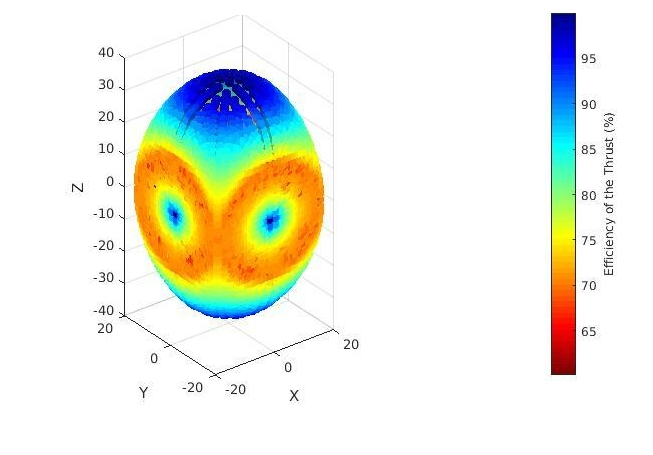
\includegraphics[width=\linewidth]{images/n=4_force.jpg}
    \caption{Force space.} \label{fig:tool_outputa}
  \end{subfigure}
  \hspace*{\fill} % separation between the subfigures
  \begin{subfigure}[b]{0.48\textwidth}
    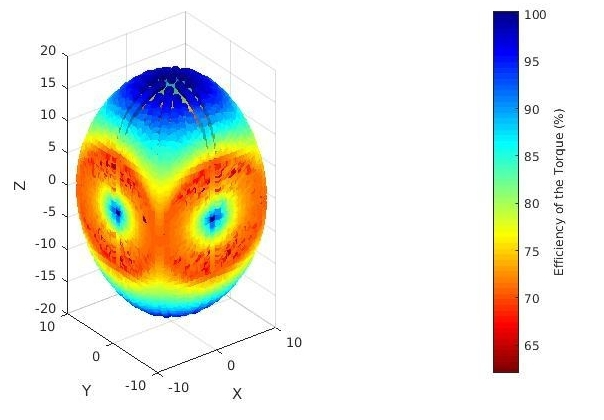
\includegraphics[width=\linewidth]{images/n=4_torque.jpg}
    \caption{Torque space.} \label{fig:tool_outputb}
  \end{subfigure}
  \hspace*{\fill} % separation between the subfigures
  \begin{subfigure}[b]{0.48\textwidth}
    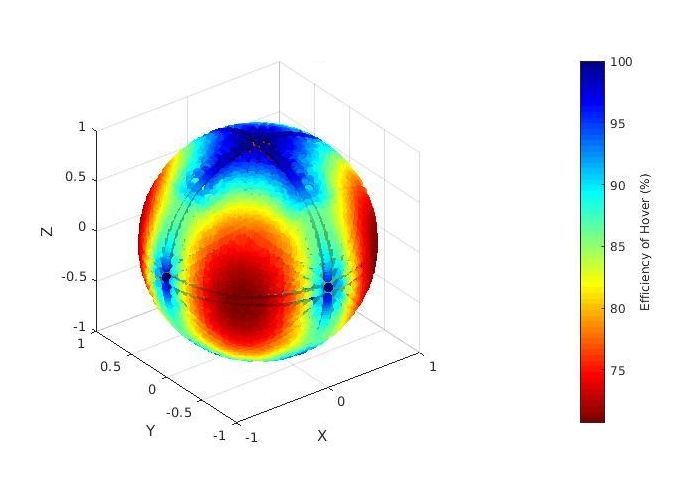
\includegraphics[width=\linewidth]{images/n=4_hover.jpg}
    \caption{Hover efficiency.} \label{fig:tool_outputc}
  \end{subfigure}
  \hspace*{\fill} % separation between the subfigures
  \begin{subfigure}[b]{0.48\textwidth}
    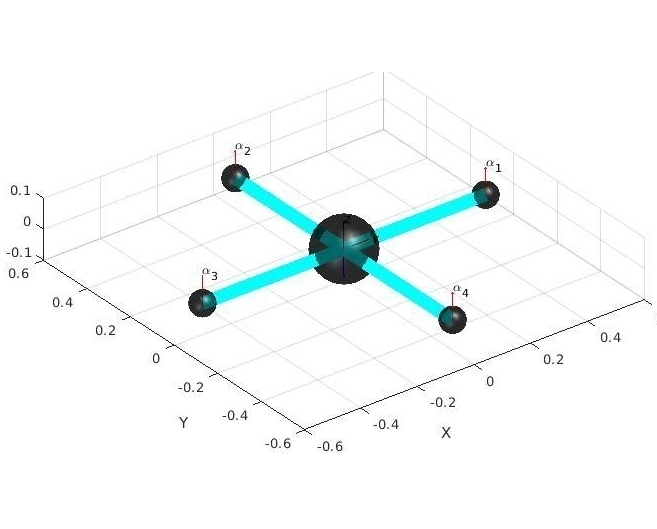
\includegraphics[width=\linewidth]{images/n=4_model.jpg}
    \caption{MAV representation.} \label{fig:tool_outputd}
  \end{subfigure}
  \caption{Example of the optimization tool's output.}
  \label{fig:tool_output}
\end{figure}

Along with the design parameters and the figure the optimization tool also
returns information on the drone capabilities called metrics. These metrics are
listed in \Cref{tab:tab_metrics}.

\begin{table}[!h]
\begin{center}
 \caption{List of the metrics returned by the optimization tool.}\vspace{1ex}
 \label{tab:tab_metrics}
 \resizebox{\textwidth}{!}{
 \begin{tabular}{|l||c|c|c|c|c|c|}
   \hline
   Metrics: & Minimal & Maximal & Mean & MAD & Task space volume & Task space surface\\ \hline \hline
   Force: & $[N]$ & $[N]$ & $[N]$ & $[N]$ & $[N^3]$ & $[N^2]$\\
   Torque: & $[Nm]$ & $[Nm]$ & $[Nm]$ & $[Nm]$ & $[N^3m^3]$ & $[N^2m^2]$\\
   Hover efficiency: & $[\%]$ & $[\%]$ & $[\%]$ & $[\%]$ & - & -\\
   \hline
 \end{tabular}}
\end{center}
\end{table}

\subsubsection{Limitations}
\label{sec:limitations}
Due to the non-linearity of the cost functions and the fact that the algorithms
available in MATLAB$^\textrm{\textregistered}$ only guarantee convergence
to local optima, the solution returned by the tool is strongly dependent on the
chosen initial solution. And also the more parameters one wants to be optimized the
more the algorithms get stuck in local optima.

\section{Simulation Approach}
\label{sec:control_approach}
As said above, a few of the optimal designs are tested in simulation on
Gazebo$^\textrm{\textregistered}$. In order to be simulated on
Gazebo$^\textrm{\textregistered}$ a robot model, which is represented
in a Unified Robot Description Format\footnote{Format based on XML used
to represent robot models in ROS} (URDF) file, is first launched on
Gazebo$^\textrm{\textregistered}$. In the mean time, a ROS node to control
the robot’s joints is also launched and the simulation can then properly start
(see \Cref{fig:sim_gazebo}).
So as to simulate the chosen optimal MAV designs, they first have to be
modeled in URDF files. Once that is done, the ROS node responsible for the
control of the MAV, that is referred to as the control node, has to be built.
The access to Voliro’s control node was luckily granted during the present work
 \citep{kamel_voliro:_2018}. Therefore, to properly control the different
design of MAV obtained, only a few changes are needed on Voliro’s control
node. First, the controller node has to be generalized for a n-rotor drone (
opposed to a 6-rotor drone for Voliro). Then, the static allocation matrix
(which is how Voliro transforms a desired angular and linear acceleration into
desired motor speeds and rotor tilting angles)
has to be generalized to a n-rotor MAV with an arbitrary arm orientation.
Finally, the arbitrary arm orientation can cause a center of mass (CoM)
offset. An additional angular acceleration thus has to be added to the desired
angular acceleration, in order to compensate for the CoM offset. This
angular acceleration is calculated as follow

\begin{equation}
  \label{com_offset}
	\dot{\omega}_{CoM} = -I_B^{-1}(R_{CoM}\times m\ddot{p}_{des})\, ,
\end{equation}

where $R_{CoM}$ is the CoM position vector and $\ddot{p}_{des}$ the desired
linear acceleration.\\
Once all these changes done, the MAV model can be controlled in
Gazebo$^\textrm{\textregistered}$ as it can be seen in \Cref{fig:sim_gazebo}).

\begin{figure}[!h]
  \centering
  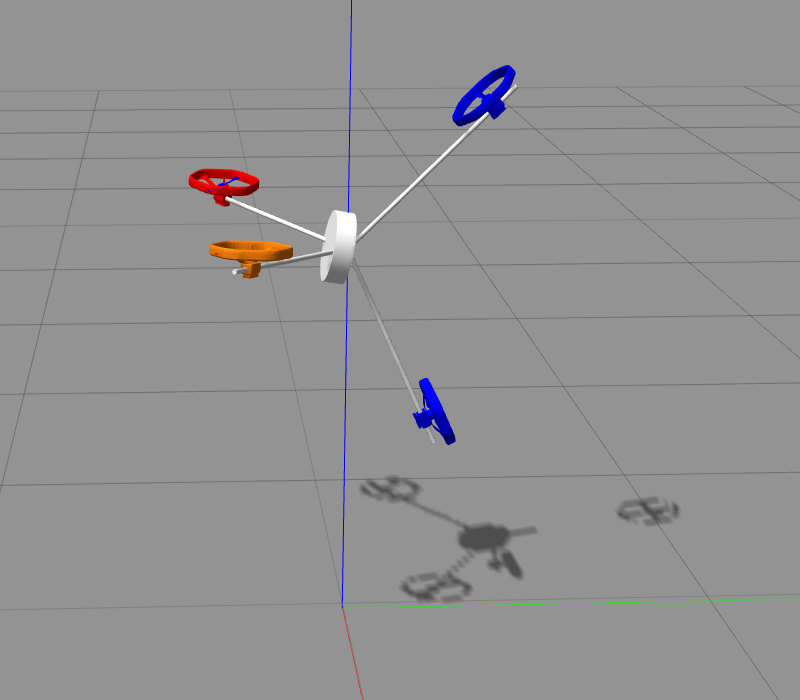
\includegraphics[width=0.45\textwidth]{images/sim_gazebo.png}
  \caption{4-rotors MAV design successfully launched and controlled in Gazebo$^\textrm{\textregistered}$.}
  \label{fig:sim_gazebo}
\end{figure}
